\subsection{Likelihood}
\label{sec:pf-likelihood}

The second component of \agls{rbm} is the update step, which incorporates the likelihood of the data into the predicted state, $p(\Vobs_k \cond{} \Vstate_k)$. In the \pf{}, as discussed in \cref{sec:pf}, updating is performed by reweighting each of the particles based on their respective likelihoods, $p(\Vobs_k \cond{} \Vstate\vi_k)$. That is,
\begin{equation}
\label{eq:vehicle_pf_update}
p(\Vstate_k \cond{} \Vobs_{1:k}) \approx
\sum_{i=1}^\Np
    \Pwt_{k}
    \DiracMeasure{\Vstate\vi_k}{\Vstate_k}
\end{equation}
where
\begin{equation}
\label{eq:vehicle_pf_reweight}
\Pwt_k = \frac{
    \Pwt_{k-1} p(\Vobs_k \cond{} \Vstate\vi_k)
}{
    \sum_{j=1}^\Np \Pwt[j]_{k-1} p(\Vobs_k \cond{} \Vstate\vi[j]_k)
}.
\end{equation}
If necessary, the particles are resampled with replacement (discussed further in \cref{sec:pf_implementation}).


The likelihood function is where the \pf{} is superior in this application. Were we to model the vehicle's state using a \kf{}, we would need to somehow compare a distribution in one dimension (distance travelled) with an observation in two dimensions (\gls{gps} coordinate). \citet{Cathey_2003} used an optimisation technique to obtain an estimated observation of distance travelled based on the observed location, which they then used as data for a \kf{}. However, as demonstrated in \cref{fig:lhood_obs}, there are situations where the ``maximised'' location may be wrong, in which case the resulting state will be erroneous.


The \pf{} effectively checks to see how plausible the observation is assuming each particle is the truth, allowing us to weight each particle by its plausibility. Since there are two types of data, two likelihood functions are required: one for \GPS{} observations, and a second for trip updates. There is no need to match the observations to distance: instead, each particle's state can be transformed into a \gls{gps} coordinate, making it directly comparable to the vehicle's reported location (see \cref{app:pf_measurement_fun}).


\subsubsection{GPS vehicle locations}
\label{sec:lhood_gps}

\begin{knitrout}\small
\definecolor{shadecolor}{rgb}{0.969, 0.969, 0.969}\color{fgcolor}\begin{figure}
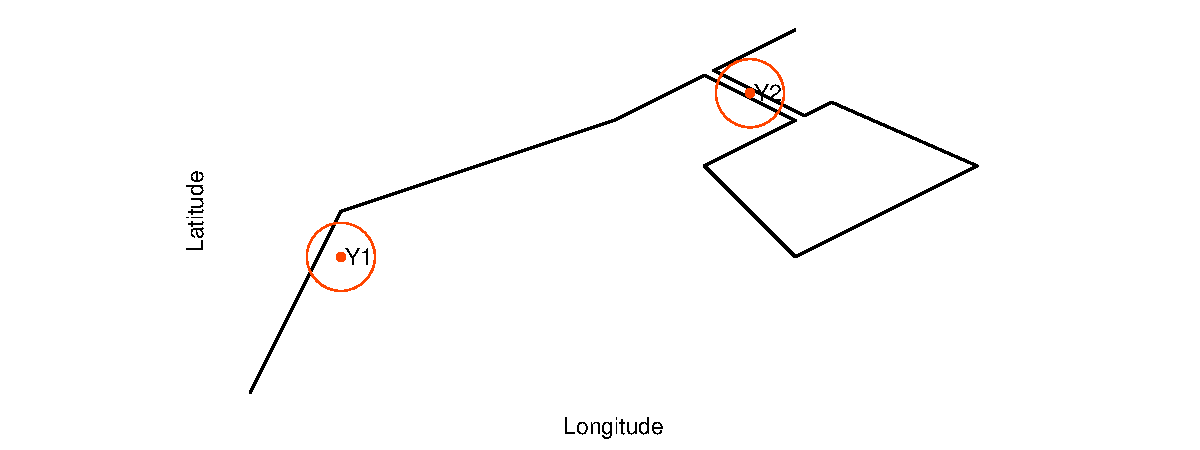
\includegraphics[width=\maxwidth]{figure/lhood_obs-1} \caption[Observations of a vehicle travelling along a path]{Observations of a vehicle travelling along a path. The red points indicate the reported GPS positions, with circles indicating the GPS error associated with each observation. Observation Y1 is easy to map to the route, while Y2 is more complicated: it could be \emph{entering} or \emph{exiting} the loop.}\label{fig:lhood_obs}
\end{figure}


\end{knitrout}





For the \gls{gps} location update, the inherent \gls{gps} error, $\GPSerr$, needs to be filtered out to get better estimates of the vehicle's state. Examples of positions are shown in \cref{fig:lhood_obs}. A particle's likelihood should represent the \emph{geographical closeness} of the estimated position to the vehicle's reported position. Therefore, we want the likelihood to depend on the \emph{distance between the observed and predicted} vehicle locations. The first step to computing the likelihood is therefore to calculate the \gls{gps} position of the \emph{particle}, $\Ppos\vi_k$, by using the \emph{measurement function},
\begin{equation}
\label{eq:pf_measurement_fun}
\Ppos\vi_k = \Vmeas(\Vstate\vi_k, \ShapePath),
\end{equation}
which is simply a deterministic function given the route's path, $\ShapePath$, a sequence of latitude-longitude pairs and the cumulative distance along the line. Details are given in \cref{app:pf_measurement_fun}. Once the geographical position of the particle is obtained, it can be compared to the observed vehicle location, as shown in \cref{fig:gps_dist}.

\begin{knitrout}\small
\definecolor{shadecolor}{rgb}{0.969, 0.969, 0.969}\color{fgcolor}\begin{figure}

{\centering 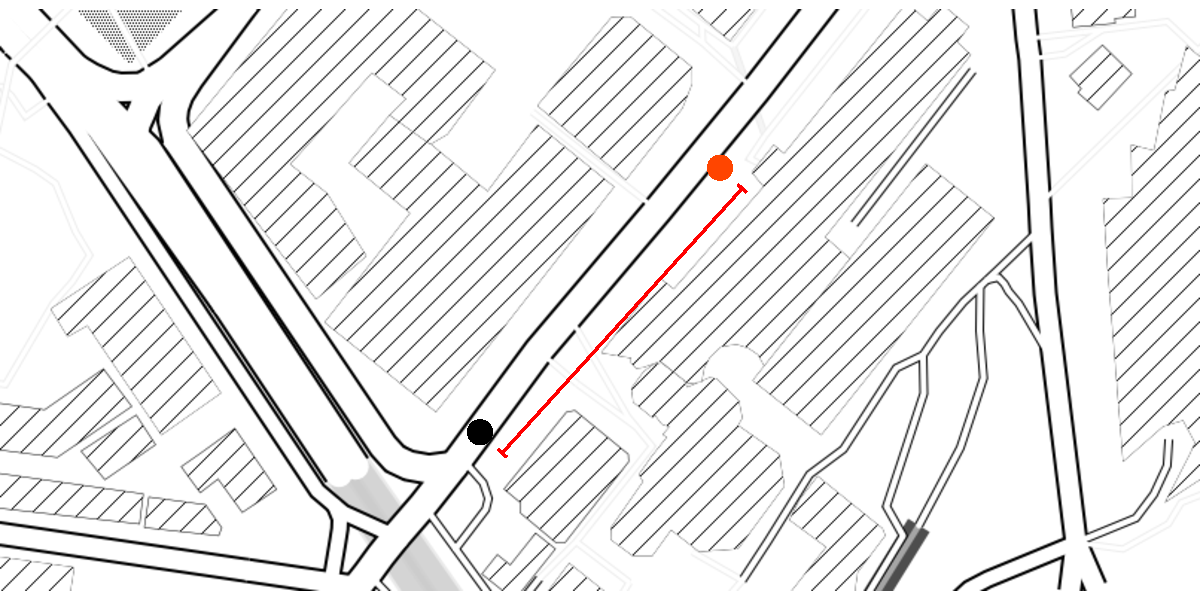
\includegraphics[width=0.8\textwidth]{figure/gps_dist-1} 

}

\caption[GPS distance between two points]{GPS distance between two points. The vehicle's reported location is shown in orange; one particle estimate of its location is in black. The desired distance is denoted by the red line.}\label{fig:gps_dist}
\end{figure}


\end{knitrout}

Computing the distance between two \gls{gps} coordinates can be achieved using several formulae, each with varying levels of accuracy. Since all the distances are going to be (very) small, the \emph{equirectangular projection} is sufficiently accurate for computing geographical distances \citep{Snyder_1998}. This projection transforms the point $\Vobs_1 = \tvec{\Vlon_1, \Vlat_1}$, where latitude $\Vlat$ and longitude $\Vlon$ are in radians (the width of one longitudinal radian depends on latitude), onto a surface with meters on both axes, centred on the point $\Vobs_0 = \tvec{\Vlon_0, \Vlat_0}$ and using the Earth's radius \mbox{$R = 6.371 \times 10^6$}~meters:
\begin{equation}
\label{eq:equirectangular_projection}
\Vproj{\Vobs_1}{\Vobs_0} =
\begin{bmatrix} x \\ y \end{bmatrix} =
R \begin{bmatrix}
(\Vlon_1 - \Vlon_0) \cos \Vlat_0 \\
(\Vlat_1 - \Vlat_0)
\end{bmatrix}.
\end{equation}
Now the distance between the points is easily computed using the \emph{euclidean distance} between their transformed coordinates,
\begin{equation}
\label{eq:obs_dist}
\dist{\Vobs_0, \Vobs_1} = \sqrt{x^2 + y^2},
\end{equation}
as shown visually in \cref{fig:gps_projection}. Note that conversion from degrees to radians is achieved by multiplying degrees by $\frac{\pi}{180}$.

\begin{knitrout}\small
\definecolor{shadecolor}{rgb}{0.969, 0.969, 0.969}\color{fgcolor}\begin{figure}

{\centering \subfloat[GPS coordinates\label{fig:gps_projection1}]{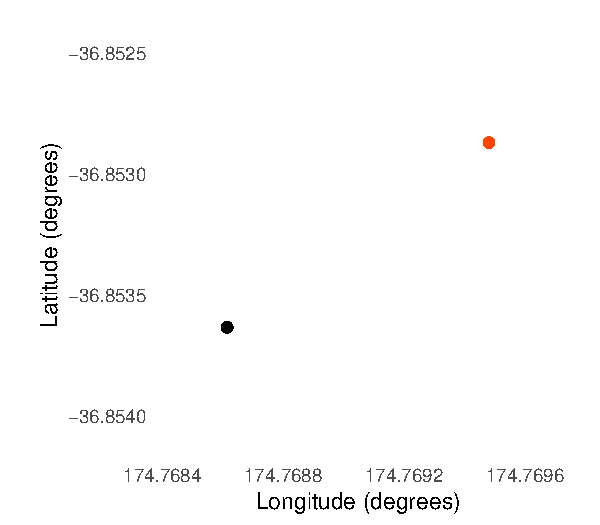
\includegraphics[width=0.49\textwidth]{figure/gps_projection-1} }
\subfloat[Projected points\label{fig:gps_projection2}]{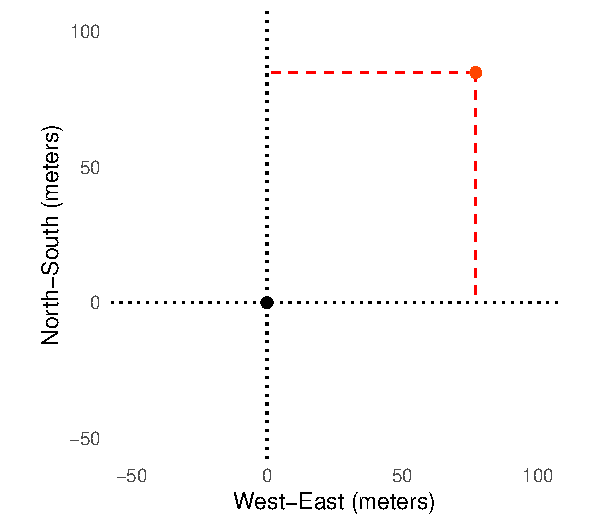
\includegraphics[width=0.49\textwidth]{figure/gps_projection-2} }

}

\caption[Equirectangular projection of GPS coordinates onto a flat surface]{Equirectangular projection of GPS coordinates ({\sc a}) onto a flat surface ({\sc b}), which allows the easy calculation of distance between a particle (black) and the vehicle's observed location (orange).}\label{fig:gps_projection}
\end{figure}


\end{knitrout}


Now that spherical observations can be compared on a flat surface, we assume that \gls{gps} observations are distributed as a multivariate random variable around the true position of the vehicle on the ground, with a \GPS{} error of $\GPSerr$, and that the variation does not depend on direction. That is, if the observation $\Vobs_k$ is projected using \cref{eq:equirectangular_projection} conditional on the true position $\Vmeas(\Vstate_k)$, then the projected point will be a multivariate random variable $\vec{r}_k \sim \Normal{\vec{0}}{\GPSerr \mat{I}}$. This can more simply be expressed by
\begin{equation}
% \label{eq:obs_projection}
\label{eq:gps_error_model}
\Vproj{\Vobs_k}{\Vmeas(\Vstate_k)} =
    \Vproj{\Vmeas(\Vstate_k)}{\Vmeas(\Vstate_k)} + \vec{r}_k
    = \vec{r}_k,
\end{equation}
and is shown graphically in \cref{fig:gps_projection2}.




From \cref{eq:equirectangular_projection,eq:obs_dist,eq:gps_error_model}, the distance between the true and observed locations is the magnitude of the error $\vec{r}_k$,
\begin{equation}
\label{eq:sq_dist}
\dist{\Vobs_k, \Vmeas(\Vstate_k)} = ||\vec{r}_k|| =
    \sqrt{r_{k1}^2 + r_{k2}^2}.
\end{equation}
However, this error can also be expressed in terms of two independent, standard Normal random variables $z_1, z_2 \sim \Normal{0}{1}$, such that $r_{jk} = \GPSerrSD z_j$ for $j = 1, 2$, leading to
\begin{equation}
\dist{\Vobs_k, \Vmeas(\Vstate_k)} =
    \sqrt{(\GPSerrSD z_1)^2 + (\GPSerrSD z_2)^2} =
    \GPSerrSD \sqrt{z_1^2 + z_2^2}.
\end{equation}
Since the distribution of two squared standard Normal random variables is $\chi^2$ distributed with 2~degrees of freedom, which is itself exponential with rate 0.5, then
\begin{equation}
\label{eq:sum_sq_dist}
z_1^2 + z_2^2 \sim \Exp{\frac{1}{2}}.
\end{equation}
Further, if $X \sim \Exp{\theta}$, then $cX \sim \Exp{\frac{\theta}{c}}$, so the squared distance is exponential with mean dependent only on the \gls{gps} error,
\begin{equation}
\label{eq:distance_distrib}
\dist{\Vobs_k, \Vmeas(\Vstate_k)}^2 \sim \Exp{\frac{1}{2\GPSerr}}.
\end{equation}

Given a particle state estimate of $\Vstate\vi_k$,
the likelihood of a \GPS{} observation using only
the distance between two coordinates is now
\begin{equation}
\label{eq:particle_lh_fun}
p(\Vobs_k \cond{} \Vstate\vi_k) =
    \frac{1}{2\GPSerr} \exp\left\{
        - \frac{\dist{\Vobs_k, \Vmeas(\Vstate\vi_k)}^2}{2\GPSerr}
    \right\},
\end{equation}
allowing the particles to be reweighted using \cref{eq:vehicle_pf_reweight}. This is shown visually in \cref{fig:pf_wts} (darker particles have greater weight), which demonstrates not only the particle reweighting by geographical proximity, but also the particle filter's innate ability to handle loops (as displayed) and other situations involving multimodality.


\begin{knitrout}\small
\definecolor{shadecolor}{rgb}{0.969, 0.969, 0.969}\color{fgcolor}\begin{figure}

{\centering 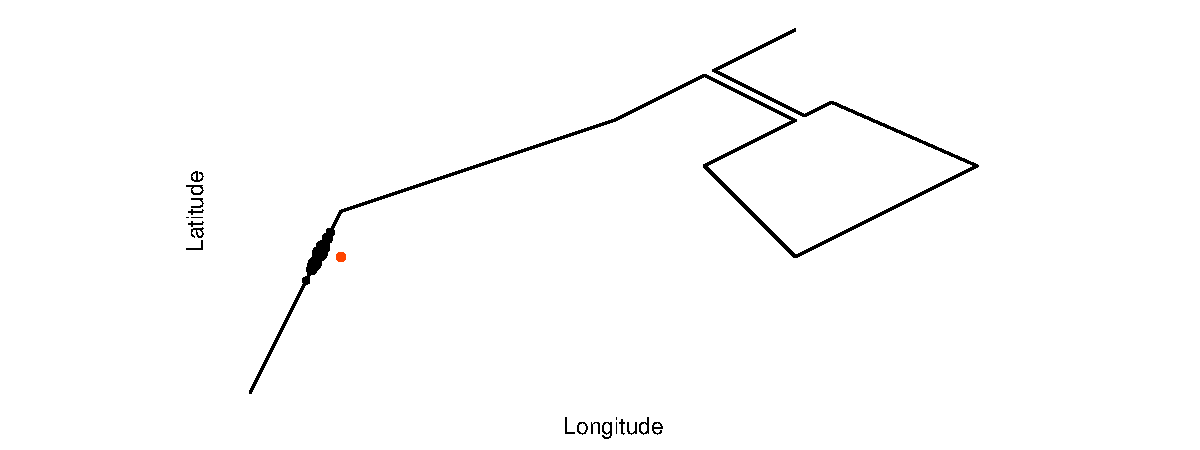
\includegraphics[width=\maxwidth]{figure/pf_wts-1} 

}

\caption[Particles are reweighted based on their geographic proximity to the vehicle's observed location]{Particles (black points) are reweighted (darker particles have more weight) based on their geographic proximity to the vehicle's observed location (red cross). There is no need to decide if the bus is going into or coming out of the loop.}\label{fig:pf_wts}
\end{figure}


\end{knitrout}


\subsubsection{Trip updates}
\label{sec:lhood_trip}

As well as vehicle position updates from \GPS{} data, \GTFS{} also provides trip updates from arrival and departure information. In many situations, it is difficult to infer a vehicle's trajectory based solely on \GPS{} data, so trip updates are an invaluable part of the update step. In this case, the \pf{} prediction step goes ahead as presented in \cref{sec:vehicle_model_trans}, but instead of comparing the coordinates, we use the arrival or departure times to compute the likelihood of the particles.


The trip update observations differ from the \GPS{} observations in that there are now three situations which may occur. The observation can be of arrival time at stop $m$, $\Varr_m$, or it can be of departure time, $\Vdep_m$. In the latter case, treatment of the observations depends on whether $\Varr_m$ was observed. This gives us three likelihood functions to derive,
\begin{itemize}
\item $p(\Varr_m \cond{} \Vstate_k)$, the arrival time likelihood function,
\item $p(\Vdep_m \cond{} \Vstate_k, \text{arrival missing})$, the departure time likelihood conditional on not having observed arrival time, and
\item $p(\Vdep_m \cond{} \Vstate_k, \text{arrival observed})$, the departure time likelihood conditional on having observed arrival time.
\end{itemize}


To compute these likelihoods, we recall the dwell time model described by \cref{eq:stop_dwell_time,eq:stop_pstop,eq:stop_total_dwell_time}. Two additional parameters are needed: the actual arrival time of the bus at stop $m$, $\Tarr_{m}$, and the measurement error of arrival time in seconds, $\TUerr$. The arrival time can be computed for each stop $m$ directly from the model (via interpolation). The departure time is then computed by summing the arrival and dwell times.


The observed arrival and departured times, denoted $\Varr_m$ and $\Vdep_m$, respectively, are modelled as Normal random variables with mean and variance determined by the described model. For arrival time, this is
\begin{equation}
\label{eq:tu_arr_lhood}
\Varr_m \sim \Normal{\Tarr_{mr}}{\TUerr},
\end{equation}
and for departure time, using dwell time $\pdwell_m$ from \cref{eq:stop_total_dwell_time}, is
\begin{equation}
\label{eq:tu_dep_lhood}
\Vdep_m \sim \Normal{\Tarr_m + \pdwell_m}{\TUerr}.
\end{equation}


In our \pf{} implementation, each observation is processed individually: in situations where more than one type of observation is recieved, they are processed in chronological order and the particles reweighted between each. The necessary likelihood component for \cref{eq:vehicle_pf_reweight} is therefore
\begin{equation}
\label{eq:tu_obs_lhood}
p(\Vobs_k \cond{} \Vstate\vi_k) =
\begin{cases}
\frac{1}{\sqrt{2\pi\TUerr}}
    \exp\left\{
        -\frac{(\Varr_m - \Tarr_m)^2}{2\TUerr}
    \right\} & \text{for arrival times,} \\
\frac{1}{\sqrt{2\pi\TUerr}}
    \exp\left\{
        -\frac{(\Vdep_m - \Tarr\vi_m - \pdwell\vi_m)^2}{2\TUerr}
    \right\} & \text{for departure times,}
\end{cases}
\end{equation}
allowing the particle sample to be reweighted according to the temporal difference in arrival and departure times as demonstrated in \cref{fig:tu_update}.

\begin{knitrout}\small
\definecolor{shadecolor}{rgb}{0.969, 0.969, 0.969}\color{fgcolor}\begin{figure}

{\centering 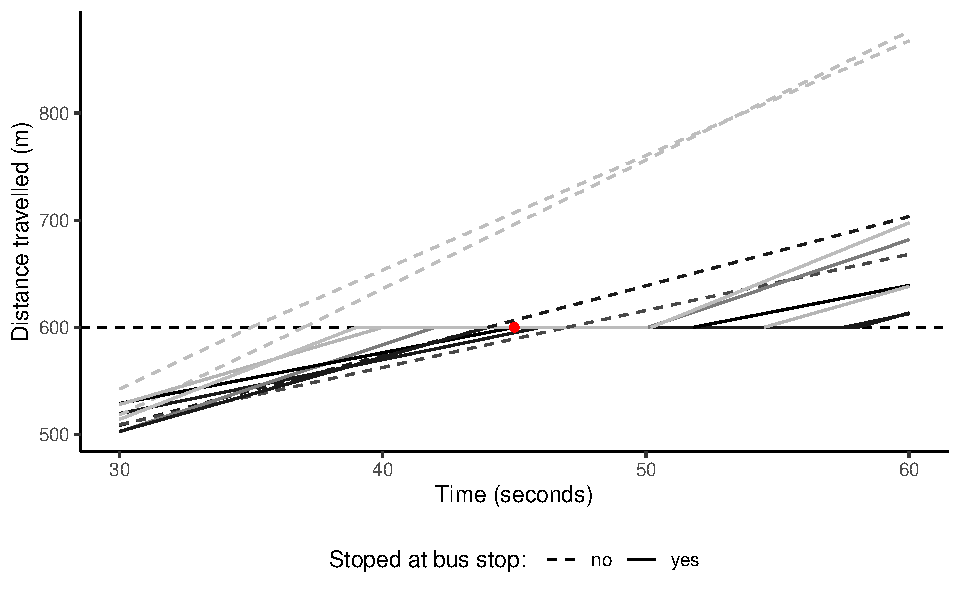
\includegraphics[width=0.8\textwidth]{figure/tu_update-1} 

}

\caption[Particles are weighted by their arrival time at a stop]{Particles travelling past a stop with an arrival time observation (red point). Solid lines represent particles that stopped, while dashed lines indicate particles that did not. Darker lines represent particles with bigger weights according to the arrival time likelihood.}\label{fig:tu_update}
\end{figure}


\end{knitrout}
